\documentclass[a4paper,14pt]{extarticle}

\usepackage[utf8x]{inputenc}
\usepackage[T1,T2A]{fontenc}
\usepackage[russian]{babel}
\usepackage{hyperref}
\usepackage{indentfirst}
\usepackage{here}
\usepackage{array}
\usepackage{graphicx}
\usepackage{caption}
\usepackage{subcaption}
\usepackage{chngcntr}
\usepackage{amsmath}
\usepackage{amssymb}
\usepackage{pgfplots}
\usepackage{pgfplotstable}
\usepackage[left=2cm,right=2cm,top=2cm,bottom=2cm,bindingoffset=0cm]{geometry}
\usepackage{multicol}
\usepackage{askmaps}
\usepackage{titlesec}
\usepackage{listings}
\usepackage{color}
\usepackage{courier}

\definecolor{green}{rgb}{0,0.6,0}
\definecolor{gray}{rgb}{0.5,0.5,0.5}
\definecolor{purple}{rgb}{0.58,0,0.82}

\lstset{
	language=Verilog,
	backgroundcolor=\color{white},   
	basicstyle=\small\ttfamily,
	commentstyle=\color{green},
	keywordstyle=\color{blue},	
	numberstyle=\tiny\color{gray},
	stringstyle=\color{purple},
	breakatwhitespace=false,
	breaklines=true,
	captionpos=b,
	keepspaces=true,
	numbers=left,
	numbersep=5pt,
	showspaces=false,
	showstringspaces=false,
	showtabs=false,
	tabsize=4,
	frame=single,
	inputpath={../quartus/},
	literate={~} {$\sim$}{1}
}

\renewcommand{\le}{\ensuremath{\leqslant}}
\renewcommand{\leq}{\ensuremath{\leqslant}}
\renewcommand{\ge}{\ensuremath{\geqslant}}
\renewcommand{\geq}{\ensuremath{\geqslant}}
\renewcommand{\epsilon}{\ensuremath{\varepsilon}}
\renewcommand{\phi}{\ensuremath{\varphi}}
\renewcommand{\thefigure}{\arabic{figure}} 	
\renewcommand*\not[1]{\overline{#1}}

\titleformat*{\section}{\large\bfseries} 
\titleformat*{\subsection}{\normalsize\bfseries} 
\titleformat*{\subsubsection}{\normalsize\bfseries} 
\titleformat*{\paragraph}{\normalsize\bfseries} 
\titleformat*{\subparagraph}{\normalsize\bfseries} 

\counterwithin{figure}{section}
\counterwithin{equation}{section}
\counterwithin{table}{section}
\newcommand{\sign}[1][5cm]{\makebox[#1]{\hrulefill}}
\graphicspath{{../pics/}}
\captionsetup{justification=centering,margin=1cm}
\def\arraystretch{1.3}
\setlength\parindent{5ex}
\titlelabel{\thetitle.\quad}

\begin{document}

\begin{titlepage}
\begin{center}
	Санкт-Петербургский Политехнический Университет Петра Великого\\[0.3cm]
	Институт компьютерных наук и технологий \\[0.3cm]
	Кафедра компьютерных систем и программных технологий\\[4cm]
	
	\textbf{ОТЧЕТ}\\ 
	\textbf{по лабораторной работе}\\[0.5cm]
	\textbf{SystemVerilog №4}\\[0.1cm]
	Автоматизация проектирования\\ дискретных устройств\\[4.0cm]
\end{center}

\begin{flushright}
	\begin{minipage}{0.45\textwidth}
		\textbf{Работу выполнил студент}\\[3mm]
		группа 33501/4 \hspace*{9mm} Дьячков В.В.\\[5mm]
		\textbf{Преподаватель}\\[5mm]
		\sign[1.5cm] \hspace*{1mm} к.т.н., доц. Филиппов А.С. \\[5mm]
	\end{minipage}
\end{flushright}

\vfill

\begin{center}
	Санкт-Петербург\\
	\the\year
\end{center}
\end{titlepage}

\addtocounter{page}{1}
\counterwithin{lstlisting}{section}

\tableofcontents
%\listoffigures
\newpage

\section{Цель работы}

\begin{itemize}
	\item Получение навыков анализа простейших процессов с использованием базовых функций встраиваемого логического анализатора SignalTap II и ISSPE-мегафункции приема и установки сигналов через JTAG в пакете Quartus II;
	\item Исследование работы варианта реализации широтно-импульсного модулятора с использованием средств системной отладки пакета Quartus II.
\end{itemize}

\section{Ход работы}

\subsection{Создание и ввод проекта}

На рис. \ref{fig:source} изображена схема исследуемого объекта -- широтно-импульсного модулятора (счетчик \code{Counter_PWM}, компаратор \code{Compare_PWM} и \code{DFF}-триггер). Счетчик работает с тактовой частотой 25МГц. Сигнал с выхода триггера подается на вывод, подключенный к \code{LED}. Рабочие данные поступают на ШИМ с входных выводов \code{D[]}.

\vspace{-0.5cm}
\begin{figure}[H]
	\begin{center}
		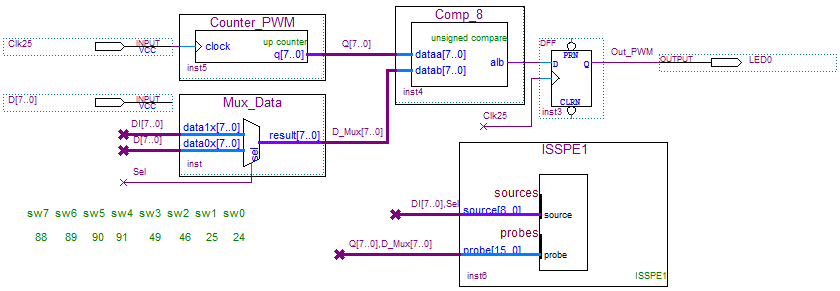
\includegraphics[width=\textwidth]{source}
		\caption{Исследуемый проект}
		\label{fig:source}
	\end{center}
\end{figure}
\vspace{-0.5cm}

Для отладки ШИМ в состав проекта введены мультиплексор данных \code{Mux_Data} и блок \code{ISSPE}, позволяющий в процессе отладки исключить системное окружение, задающее сигналы на выводы \code{D[]}. Данные на компаратор поступают с выхода мультиплексора \code{Mux_Data}, который в соответствии с управляющим сигналом \code{Sel} коммутирует на свой выход либо внешние данные \code{D[]} (сигналы на \code{D[]} подаются с переключателей \code{SW[7..0]}), либо внутреннюю шину данных \code{DI[]}. При отладке ШИМ на лабораторном стенде создание управляющего сигнала \code{Sel} и формирование кода на внутренней шине данных \code{DI[]} обеспечивается с помощью мегафункции In-System Sources and Probe Editor (ISSPE). ISSPE также подключен для наблюдения сигналов на входах компаратора (\code{Q[]}, \code{D_Mux[]}).

\subsection{Компиляция проекта}

Выполним компиляцию введенного проекта и проанализируем предупреждения. Полученные предупреждения говорят о том, что не найден файл, задающий временные ограничения. В листинге \ref{code:sdc} приведен созданный SDC файл.

\begin{lstlisting}[caption=Synopsys Design Constraints (SDC) файл, label=code:sdc]
create_clock -name Clk25 -period 40.000 [get_ports {Clk25}]
derive_clock_uncertainty
\end{lstlisting}

После компиляции предупреждения не появлются. Определим аппаратурные затраты и быстродействие проекта:

\begin{enumerate}
	\item Аппаратурные затраты: 905 ЛЭ, включая 688 триггеров;
	\item Быстродействие Slow 1200 mV 85C Model:
		\begin{itemize}[leftmargin=*]
			\item \code{altera_reserved_tck}: Fmax = 72.85 MHz, Restricted Fmax = 72.85 MHz
			\item \code{Clk25}: Fmax = 146.43 MHz, Restricted Fmax = 146.43 MHz
		\end{itemize}
\end{enumerate}

\subsection{Настройка In System Sources and Probe Editor}

Сгруппируем вывода в In System Sources and Probe Editor так, как показано на рис. \ref{fig:isspe1}.

\vspace{-0.5cm}
\begin{figure}[H]
	\begin{center}
		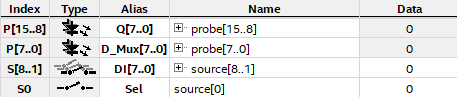
\includegraphics[scale=1]{isspe1}
		\caption{Настройка In System Sources and Probe Editor}
		\label{fig:isspe1}
	\end{center}
\end{figure}
\vspace{-0.5cm}

\subsection{Подготовка логического анализатора SignalTapII}

Создадим экземпляр логического анализатора \code{ELA1} и зададим настройки в соответствии с рис. \ref{fig:stp1}. Аппаратные затраты для реализации созданного анализатора: 862 логических элемента, 34816 бит памяти, 4 medium blocks.

\begin{figure}[H]
	\begin{center}
		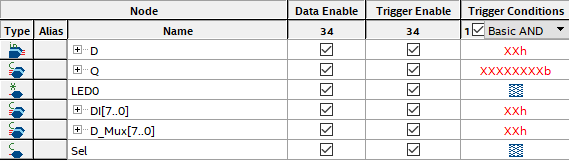
\includegraphics[scale=1]{stp1}
		\caption{Настройка Signal Tap Logic Analyzer}
		\label{fig:stp1}
	\end{center}
\end{figure}
\vspace{-0.5cm}

\subsection{Исследование работы ШИМ в системе-прототипе}

На рис. \ref{fig:stp2} приведена диаграмма, подтверждающая работоспособность счетчика ШИМ.
\begin{figure}[H]
	\begin{center}
		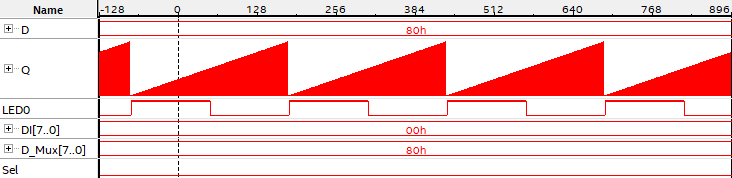
\includegraphics[width=\textwidth]{stp2}
		\caption{Проверка работоспособности счетчика ШИМ}
		\label{fig:stp2}
	\end{center}
\end{figure}
\vspace{-0.5cm}

Проверим работоспособность ШИМ в In System Sources and Probe Editor.
\begin{figure}[H]
	\centering
	\begin{subfigure}[b]{\textwidth}
		\centering
		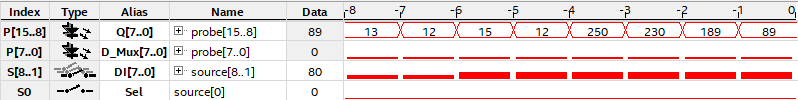
\includegraphics[width=\textwidth]{isspe2}
		\vspace{0.2cm}
	\end{subfigure}
	\begin{subfigure}[b]{\textwidth}
		\centering
		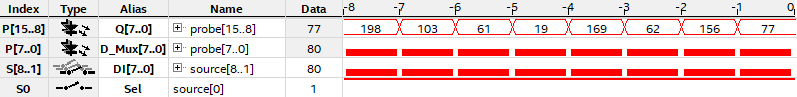
\includegraphics[width=\textwidth]{isspe3}
		\vspace{0.2cm}
	\end{subfigure}
	\begin{subfigure}[b]{\textwidth}
		\centering
		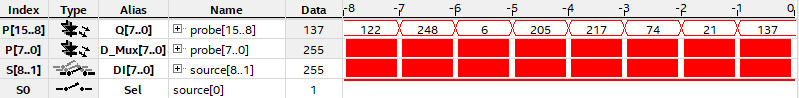
\includegraphics[width=\textwidth]{isspe4}
	\end{subfigure}
	\caption{Проверка работоспособности счетчика ШИМ в ISSPE}
	\label{fig:isspe2}
\end{figure}

Если \code{Sel = 0}, то входные данные считываются из положения переключателей \code{SW[7..0]}. Если \code{sel = 1}, то входные данные задаются в редакторе ISSPE в значении \code{DI[7..0]}. Выход синтезированной схемы соединен с \code{LED[0]}, следовательно ШИМ регулирует яркость светодиода: чем меньше значение \code{DI[7..0]} (более узкий импульс), тем ярче горит светодиод.

\subsection{Исследование ШИМ с использованием сегментированного буфера логического анализатора}

Для управления ШИМ будем использовать код, формируемый генератором линейно растущего, а затем линейно уменьшающегося кода. Генератор реализуется на основе реверсивного счетчика \code{Cnt_Triangle}, структура которого приведена на рис. \ref{fig:source2}.
\begin{figure}[H]
	\begin{center}
		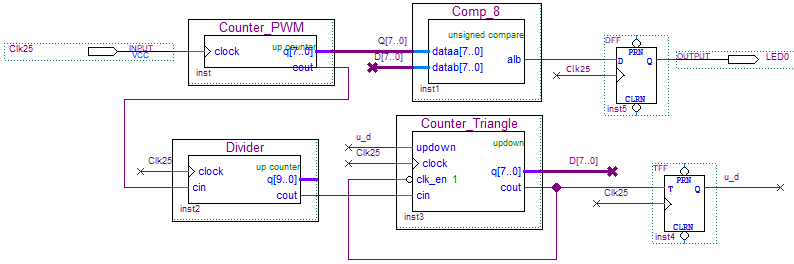
\includegraphics[width=\textwidth]{source2}
		\caption{Схема проекта с защитой от дребезга контактов}
		\label{fig:source2}
	\end{center}
\end{figure}

Настроим логической анализатор как на рис. \ref{fig:stp3}.
\begin{figure}[H]
	\begin{center}
		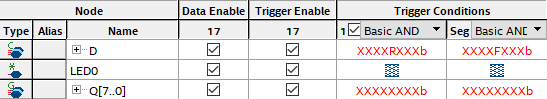
\includegraphics[scale=1]{stp3}
		\caption{Схема проекта с защитой от дребезга контактов}
		\label{fig:stp3}
	\end{center}
\end{figure}

На рис. \ref{fig:stp4} приведены захваченные данные в Signal Tap Logic Analyzer.
\begin{figure}[H]
	\centering
	\begin{subfigure}[b]{\textwidth}
		\centering
		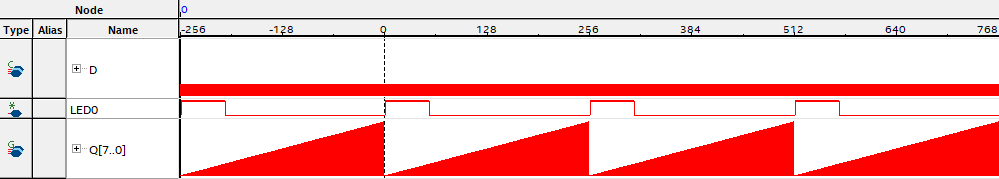
\includegraphics[width=\textwidth]{stp4}
		\vspace{0.2cm}
	\end{subfigure}
	\begin{subfigure}[b]{\textwidth}
		\centering
		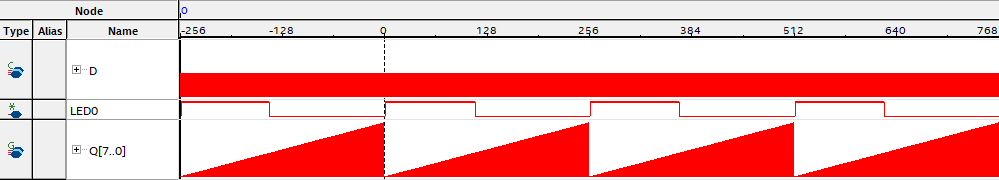
\includegraphics[width=\textwidth]{stp5}
		\vspace{0.2cm}
	\end{subfigure}
	\begin{subfigure}[b]{\textwidth}
		\centering
		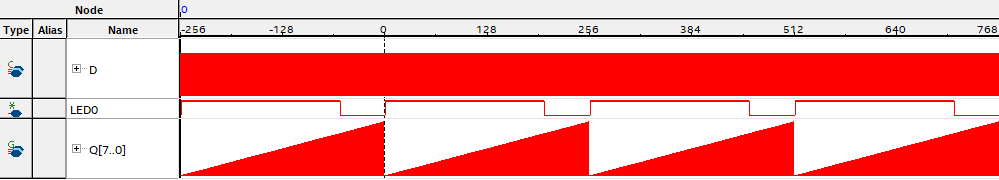
\includegraphics[width=\textwidth]{stp6}
	\end{subfigure}
	\caption{Захват данных данные в SignatlTapII}
	\label{fig:stp4}
\end{figure}

%На рис. \ref{fig:stp7} изображен захват данных с использованием сегментированного буфера с таким условием захвата, чтобы отобразить 32 значения длительности выходного сигнала за период управления яркостью свечения светодиода.
%\begin{figure}[H]
%	\begin{center}
%		\includegraphics[scale=1]{stp7}
%		\caption{Захват данных с использованием сегментированного буфера}
%		\label{fig:stp7}
%	\end{center}
%\end{figure}

\section{Выводы}

Для изучения ШИМ использован встроенный логический анализатор SignalTapII и средство In System Sources and Probe Editor. Исследовалась схема с возможностью выбора входных данных для счетчика ШИМ. ISSPE позволяет задавать входные сигналы схемы прямо из QuartusII и схема ШИМ с входными данными, поступающими со счетчика, генерирующего треугольный сигнал. Для достижения цели исследования ШИМ были решены следующие задачи: исследование работы в системе-прототипе, а также исследование с использованием сегментированного буфера логического анализатора путем задания необходимых условий захвата.

\end{document}